\chapter{Diffusion Model}
\section{Introduction}

	(Denoising) Diffusion models have emerged as the new SOTA family of deep generative models. 
	\begin{itemize}
		\item First proposed in 2015.
		\item Outperform GANs on image synthesis (DDPM) $\sim$ 2020.
		\item Stable training dynamics.
		\item Image synthesis, super resolution, text-to-image, and so on.
%		\item DMs are inspired by non-equilibrium thermodynamics. 
%			\begin{itemize}
%				\item Random motion of molecules from a region of high concentration to a region of low concentration.
%			\end{itemize}
	\end{itemize}
%	\begin{figure}[h]
%		\centering
%		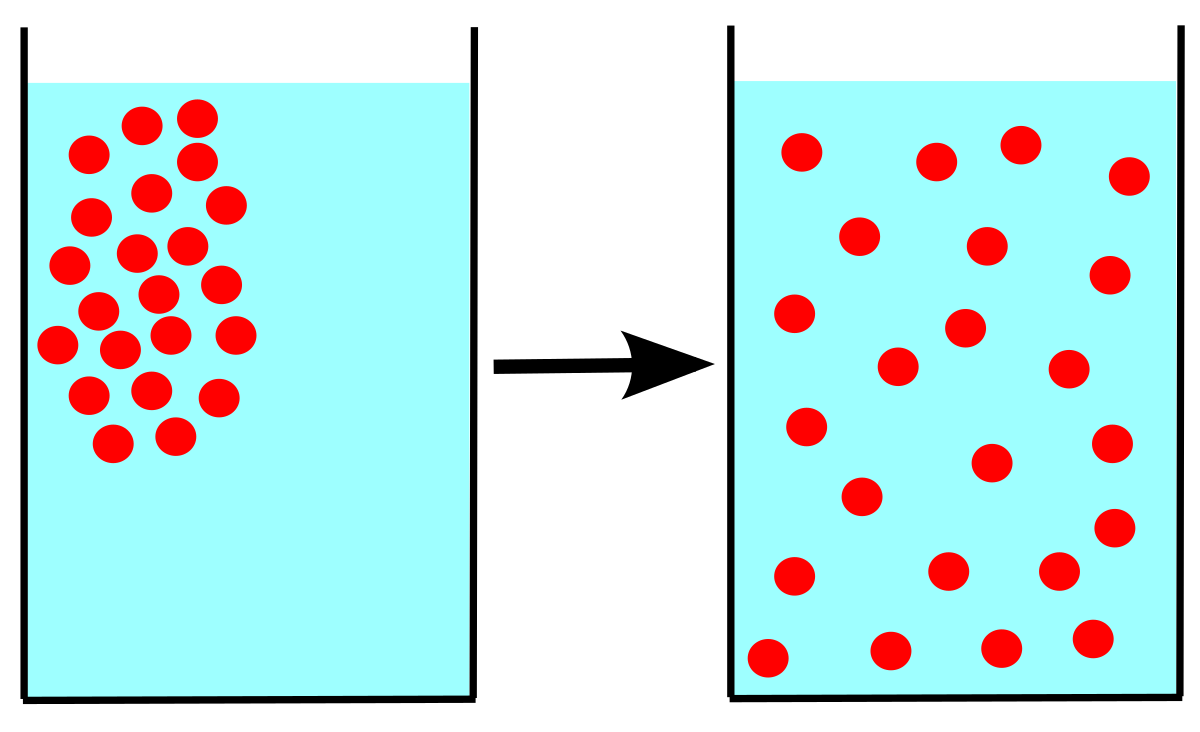
\includegraphics[scale=0.15]{./images/diffusion.png}
%		\caption{Disffusion.}
%		\label{fig:diffusion}
%	\end{figure}
% \vskip0pt plus 1filll
% \href{https://arxiv.org/abs/1503.03585}{\tiny \blue{ICML 2015 Deep Unsupervised Learning using Nonequilibrium Thermodynamics}}

	The overall idea is to construct a Markov chain of progressively less noisy samples. Each transition denoises a noisy sample. Diffusion models consist of two Markov chains:
	\begin{enumerate}
		\item Forward: A Markov chain of diffusion steps to \textbf{slowly add random noise} to data. 
			$$\rvx_0\to \rvx_1\cdots\to \rvx_T$$
		\item Backward (Reverse): Learn to \textbf{reverse the diffusion process} to construct desired data samples from the noise. 
			$$\rvx_T\to \rvx_{T-1}\cdots\to \rvx_0$$
	\end{enumerate}
	\begin{figure}[t]
		\centering
		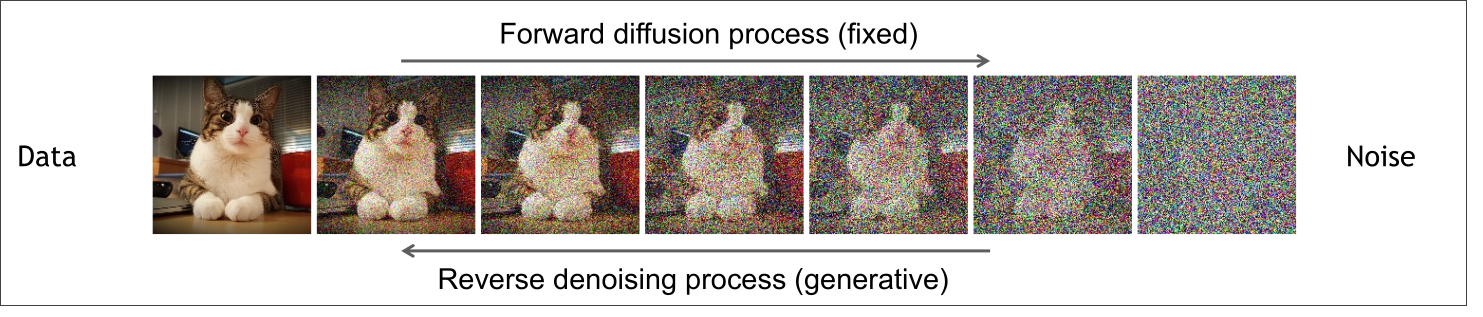
\includegraphics[scale=0.28]{./images/diffusion/diffusion_model.png}
	\end{figure}
	% \href{https://cvpr2022-tutorial-diffusion-models.github.io/}{\tiny \blue{CVRP 2022 Tutorial: Denoising Diffusion-based Generative Modeling: Foundations and Applications}}

\textbf{Some properties of diffusion models}:
	\begin{enumerate}
		%$$q(\rvx_t|\rvx_{t-1}) = \mathcal{T}(\rvx_t|\rvx_{t-1})$$
		\item Diffusion model has a pre-defined sampling equation.
			\begin{itemize}
				\item The equation relies on a random noise.
				\item Noise is all we need $\to$ Predict noise at a time step $t$.
			\end{itemize}
		\item Fit a model via forward and backward processes.
		\item \textbf{Iterative transform} of one distribution into another via \textbf{Makov Chain}.
			\begin{itemize}
				\item $\mathcal{D}_{data}\to \mathcal{N}$.
				\item $\mathcal{N}\to \mathcal{D}_{data}$.
				\item Diffusion model$\approx$Generative Markov Chain.
			\end{itemize}
		\item Learn a transition model:
			$$p_\theta(\mathbf{x}_{t-1}|\rvx_t) = \mathcal{N}(\mathbf{x}_{t-1}|\boldsymbol{\mu}_{\theta}(\mathbf{x}_{t}, t), \boldsymbol{\Sigma}_\theta(\mathbf{x}_t,t)).$$
		\item Base case: $p(\mathbf{x}_T) = \mathcal{N}(0,I)$ 
		\item Marginal distribution over $\mathbf{x}_0$:
			$$p_\theta(\mathbf{x}_0) = \int p_\theta(\rvx_0,\dots,\mathbf{x}_T)d\rvx_1,\dots,\rvx_T$$
		\item We want to learn the parameters so that
			$$p(\rvx_0)\approx p_\theta(\rvx_0)$$

	\end{enumerate}

\section{Forward Diffusion}

	\begin{itemize}
		\item We want to model a forward trajectory (by the Markov property): 
			$$q(\mathbf{x}_{0:T}) = q(\rvx_0)\prod^T_{t=1} \underbrace{q(\mathbf{x}_t \vert \mathbf{x}_{t-1})}_{\text{Transition kernel}} $$
		\item Slow transform with a large $T$: $\rvx_0\to \rvx_1\cdots\to \rvx_T$
			\begin{itemize}
				\item Imagine someone said he is from Germany.
				\item We can't exactly track his journey without more information.
				\item We need to add more steps!
			\end{itemize}
		\item How to model $q(\mathbf{x}_t \vert \mathbf{x}_{t-1})$?
%		\item By the Markov property, $q$ is given by
%			$$q(\mathbf{x}_{1:T} \vert \mathbf{x}_0) &=  \prod^T_{t=1} q(\mathbf{x}_t \vert \mathbf{x}_{t-1})$$
		%\item $q(\mathbf{x}_t \vert \mathbf{x}_{t-1}) = $
	\end{itemize}

Forward Diffusion: $q(\rvx_t \vert \rvx_{t-1})$
	In a continuous case (\eg image), each transition can be parameterized as follows:
\begin{align}
	q(\rvx_t \vert \rvx_{t-1}) &= \mathcal{N}(\mathbf{x}_t; \sqrt{1 - \beta_t} \rvx_{t-1}, \beta_t\mathbf{I})
	\label{eq:forward_diffusion}
\end{align}
\begin{itemize}
		\item $\beta_t\in (0,1)$ is a variance at time $t$.
		\item $\sqrt{1 - \beta_t}$ downscales $\rvx_{t-1}$ to be 0, $\beta_1<\cdots<\beta_t$. Thus, $\rvx_t$ will become more noisier. $\rvx_t$ can be sampled as:
			$$\mathbf{x}_t= \sqrt{1 - \beta_t} \mathbf{x}_{t-1}+ \sqrt{\beta_t} \odot \epsilon$$
			\begin{enumerate}
				\item Sample $\rvx_{t}\sim q(\rvx_t)$ and scale it by $\sqrt{1 - \beta_t}$
				\item Adds noise $\epsilon\sim \mathcal{N}(0,I)$ with variance $\beta_t$.
			\end{enumerate}
		\item The above process is autoregressive (\ie ancestral sampling), but we can sample $\mathbf{x}_t$ directly from $q(\mathbf{x}_t|\rvx_0)$ in an analytic form:
\begin{align}
	\rvx_t &= \sqrt{1 - \beta_t} \mathbf{x}_{t-1}+ \sqrt{\beta_t} \odot \epsilon_{t-1}\\
						   &= \sqrt{\alpha_t} \mathbf{x}_{t-1}+ \sqrt{1-\alpha_t} \odot \epsilon_{t-1}\\
						   &= \sqrt{\alpha_t} \bigg(\sqrt{\alpha_{t-1}} \mathbf{x}_{t-2}+ \sqrt{1-\alpha_{t-1}} \odot \epsilon_{t-2}\bigg) + \sqrt{1-\alpha_t} \odot \epsilon_{t-1}\\
						   &= \sqrt{\alpha_t\alpha_{t-1}} \mathbf{x}_{t-2} + \sqrt{\alpha_t-\alpha_t\alpha_{t-1}} \odot \epsilon_{t-2} + \sqrt{1-\alpha_t} \odot \epsilon_{t-1}\\
						   &= \sqrt{\alpha_t\alpha_{t-1}} \mathbf{x}_{t-2} + \sqrt{\alpha_t-\alpha_t\alpha_{t-1}+1-\alpha_t} \odot \epsilon_{t-2} \\
						   &= \sqrt{\alpha_t\alpha_{t-1}} \mathbf{x}_{t-2} + \sqrt{1-\alpha_t\alpha_{t-1}} \odot \epsilon_{t-2} \\
						   &= \dots\\
						   &= \sqrt{\prod_{t}\alpha_t} \mathbf{x}_{0} + \sqrt{1-\prod_t \alpha_t} \odot \epsilon_{t_0} \\
						   &= \sqrt{\bar{\alpha}_t} \mathbf{x}_{0}+ \sqrt{1-\bar{\alpha}_t} \odot \epsilon\\
	&\sim \mathcal{N}(\mathbf{x}_t; \sqrt{\bar{\alpha}_t} \rvx_{0}, (1-\bar{\alpha}_t)\mathbf{I}),
	% &= q(\mathbf{x}_t|\rvx_{0}), 
	\label{eq:diffusion_forward_sampling}
\end{align}
			where $\alpha_t = 1-\beta_t$ and $\bar{\alpha}_t = \prod_{s=1}^t \alpha_s$. Thus, $\mathbf{x}_t= \sqrt{\bar{\alpha}_t} \mathbf{x}_{0}+ \sqrt{1-\bar{\alpha}_t} \odot \epsilon$. Note that the fifth step is done by using the property of sum of two Gaussian distributions (\eg $\mathcal{N}(0, \sigma_1^2I)+\mathcal{N}(0, \sigma_2^2I) = \mathcal{N}(0, (\sigma_1^2+\sigma_2^2)I)$ ). 
\end{itemize}

We can get some intuitions:
\begin{itemize}
	\item The original input $\rvx_0$ \textbf{gradually loses all info} during the forward diffusion process.
	\item This Markov chain has a \textbf{stationary distribution}: As $t\to \infty$, $q(\rvx_t) \approx \mathcal{N}(0,I)$.
		\begin{itemize}
			\item In practice, $T$ is a very high number \eg 1,000.
			\item Minimize info loss for each step.
			\item Allow a smooth training.
		\end{itemize}
\end{itemize}

%\begin{frame}{Forward Diffusion: $q(\rvx_t)$}
%	\begin{align*}
%		\underbrace{q(x_t)}_{\text{diffused data dist.}} = \int \underbrace{q(x_t,x_0)}_{\text{Joint dist.}} dx_0 = \int \underbrace{q(x_0)}_{\text{Input dist.}}\underbrace{q(x_t|x_0)}_{\text{Diffusion kernel}} dx_0 .
%	\end{align*}
%	\begin{itemize}
%		\item We can sample $\rvx_t\sim q(\rvx_t)$ by first sampling $\rvx_0\sim q(\rvx_0)$
%		\item Sample $\rvx_t$ at any arbitrary noise level without iterative computations.
%		\item $\rvx_t = \sqrt{\bar{\alpha}_t}\rvx_0+\sqrt{(1-\bar{\alpha}_t)}\epsilon$ : reparameterization
%		\item $\alpha_t:=1-\beta_t$
%		\item $\bar{\alpha}_t:=\prod_{i=1}^t\alpha_i$
%		\item \red{Why sampling $\rvx_t$?}
%	\end{itemize}
%\end{frame}

%\begin{frame}{Forward Diffusion}
%	\begin{itemize}
%		\item Diffusion kernel: 
%			$$q(x_t|x_0) = \mathcal{N}(\sqrt{\bar{\alpha}_t}x_0, (1-\bar{\alpha}_t)I )$$
%		\item[] $\approx$ Gaussian convolution.
%		\item We can sample $x_t$ by adding scaled noise to $x_0$.
%		\item $\beta_t$ value is scheduled to be $\bar{\alpha}_T\to 0$ and $q(x_t|x_0)\approx \mathcal{N}(x_T;0,I)$
%	\end{itemize}
%\end{frame}



\section{Backward Process}

Generative Learning by Denoising:
	\begin{itemize}
		\item Now we know how to model the forward process (diffusion process).
		\item However, a noisy image is not what we want.
		\item We want to generate a new image with high quality.
	\end{itemize}

	How to generate data? If we can reverse the forward process, then we can draw a true sample. We call it \textbf{Backward process}!
	\begin{itemize}
		\item Start from $q(\rvx_T)\approx \mathcal{N}(0,I)$.
		\item Sample $\rvx_T\sim \mathcal{N}(\rvx_T|0,I)$
			\begin{itemize}
				\item Sample a noise vector from a prior distribution.
			\end{itemize}
		\item Iteratively sample $\rvx_{t-1}\sim q(\rvx_{t-1}|\rvx_t).$ 
			\begin{itemize}
				\item $q(\rvx_{t-1}|\rvx_t)$: \textbf{true denoising distribution} (we don't know).
			\end{itemize}
		\item In general, $q(\rvx_{t-1}|\rvx_t)$ is intractable.
		%\item In general, $q(x_{t-1}|x_t)\propto q(x_{t-1})q(x_t|x_{t-1})$ is intractable.
		\item We can \textbf{approximate} $q(\rvx_{t-1}|\rvx_t)$ as \textbf{Normal distribution} if $\beta_t$ is small in each forward diffusion step.
			\begin{itemize}
				\item \eg $\rvx_3$ to $\rvx_2$
			\end{itemize}
	\end{itemize}
	\begin{figure}[h]
		\centering
		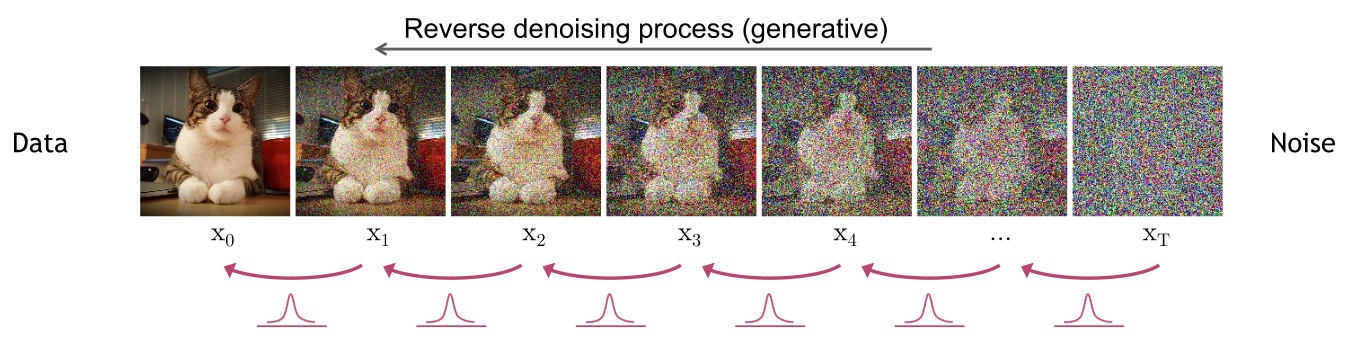
\includegraphics[scale=0.30]{./images/diffusion/reverse.png}
	\end{figure}
	\href{https://cvpr2022-tutorial-diffusion-models.github.io/}{\tiny \blue{CVPR 2022 Tutorial: Denoising Diffusion-based Generative Modeling: Foundations and Applications}}

Backward Process
	\begin{itemize}
%		\item Reverse the forward process
%			\begin{itemize}
%					\item Sample from the \textbf{exact reverse distribution} $q(\rvx_{t-1}|\rvx_t)$ (true denoising dist.), 
%					\item Recreate the true sample from a Gaussian noise input $\rvx_T\sim \mathcal{N}(0,I)$.
%				\end{itemize}
		%\item The reversal of the disffusion process has the identical form as the forward process.
		%\item The longer the trajectory the smaller the diffusion rate $\beta$ can be made.
		\item Approximate $q(\rvx_{t-1}|\rvx_t)$ using a neural network, $p_\theta(\mathbf{x}_{t-1} \vert \mathbf{x}_t)$.
		\item Backward process: $p_\theta(\mathbf{x}_{0:T}) = p(\mathbf{x}_T) \prod^T_{t=1} p_\theta(\mathbf{x}_{t-1} \vert \mathbf{x}_t)$.
			\begin{itemize}
				\item $p(\rvx_T) = \mathcal{N}(\rvx_T;0,I)$.
				\item $p_\theta(\mathbf{x}_{t-1} \vert \mathbf{x}_t) = \mathcal{N}(\mathbf{x}_{t-1}; \boldsymbol{\mu}_\theta(\mathbf{x}_t, t), \boldsymbol{\Sigma}_\theta(\mathbf{x}_t, t))$.  

				\item We can model the denoising distribution as Normal distribution like above (\cf \Cref{eq:diffusion_kl_true_denoising}).
				\item Note that the reverse conditional probability $q(\rvx_{t-1}|\rvx_t)$ is tractable when it is conditioned on $\rvx_0$ as shown in \Cref{eq:diffusion_kl_true_denoising}. This allows us to train a neural network to model this denoising distribution. 
			\end{itemize}
			% \begin{itemize}
			% 	\item Network outputs mean and variance ($\boldsymbol{\mu}_{\theta}$ and $\boldsymbol{\Sigma}_{\theta}$). 
			% 	\item We are not going to make a model to predict them directly.
			% 	\item \textbf{Train a noise prediction network.}
			% \end{itemize}
		\item Key to the success of this sampling process is training the reverse Markov chain to match the actual time reversal of the forward Markov chain. 
		\item After optimizing the backward process, the sampling procedure is that just sample Gaussian noise from $p(\rvx_T)$ and then iteratively running the denoising transitions (backward process) for T steps to generate a novel $\rvx_0$.
	\end{itemize}

